\documentclass{beamer}

\usepackage[utf8]{inputenc}
\usepackage{amssymb}
\usepackage{graphicx}
\graphicspath{ {figs/} }



\title{Efficient, Feature-based, Conditional Random Field Parsing}
\author{Paper by: Jenny Rose Finkel, Alex Kleeman, Christopher D. Manning}
\institute{Published at ACL, 2008}
\date{}


\begin{document}


\begin{frame}
  \titlepage
  Presentation by: Michael Zhang
\end{frame}



\begin{frame}
  \frametitle{Overview}

  \begin{block}{Constituency Parsing}
    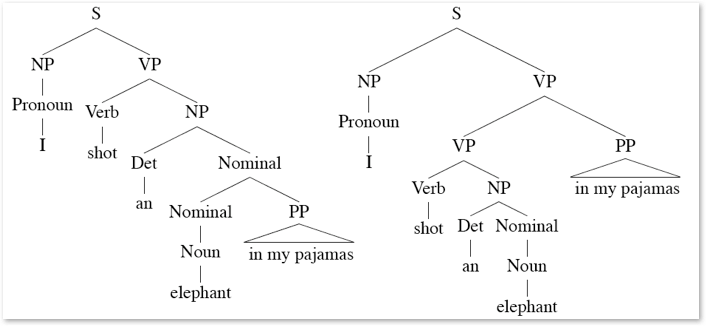
\includegraphics[width=4in]{example_parse.png}
  \end{block}

  \begin{block}{Objective}
    Given some sentence $S$, assign some parse tree $T$.
  \end{block}

\end{frame}


\begin{frame}
  \frametitle{Overview}

  \begin{block}{Objective}
    Given some sentence $S$, assign some parse tree $T$.
  \end{block}

  \begin{itemize}
    \item Parsing models at the time were dominated by \textbf{generative} methods
    \item However, \textbf{discrimitive} models had been shown to outperform generative models
          in other NLP tasks
    \begin{itemize}
      \item Discrimitive models have not surpassed generative models due to the computational
            complexity of the task
    \end{itemize}
  \end{itemize}

\end{frame}


\begin{frame}
  \frametitle{Overview}

  Prior work on discrimitive parsing fell into 3 categories:
  \begin{itemize}
    \item Reranking n-best outputs from a generative parser
    \item Parse by making a series of independent, discriminative decisions using either greedy
          search or beam search.
    \item Perform joint inference via dynamic programming algorithms for training and to
          find the globally best parse
    \begin{itemize}
      \item Previous work in this vein has been limited to shorter sentences, or giving up
            on features
    \end{itemize}
  \end{itemize}

\end{frame}

\begin{frame}
  \frametitle{Overview}

  \begin{block}{Contribution}
    \begin{itemize}
      \item Created a feature based, discriminative model for parsing
      \item Made a practical CRF model that could be easily trained and perform on longer sentences
    \end{itemize}
  \end{block}

\end{frame}

\begin{frame}
  \frametitle{The model: CRF-CFG}

  \begin{block}{Context Free Grammar}
    Consits of set of terminals $\{w^k\}$, non-terminals $\{N^k\}$, start symbol $\{ROOT\}$,
    rules $\{\rho = N^i \rightarrow \zeta^i\}$
    
  \end{block}

  \vspace{.25in}
  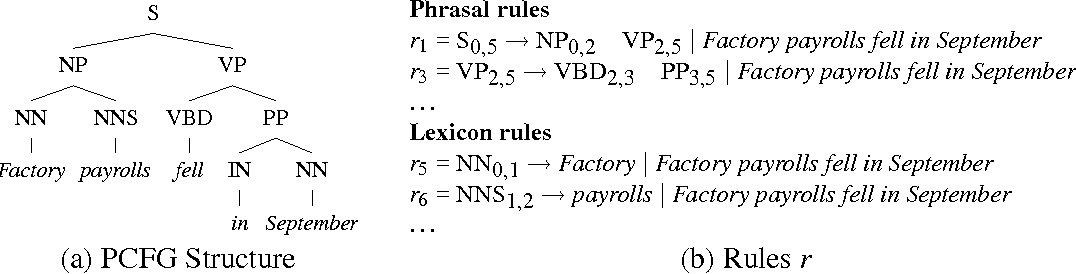
\includegraphics[width=3in]{crfcfg.png}

  \begin{block}{CRF-CFG}
    \begin{itemize}
      \item Defines local potentials $\phi(r | s; \theta)$
    \end{itemize}
    $$P(t | s ; \theta) = \dfrac{1}{Z_s} \prod_{r \in t} \phi(r | s; \theta)$$
    $$Z_s = \sum_{t \in \tau(s)} \prod_{r \in t} \phi(r | s; \theta)$$
  \end{block}


\end{frame}

\begin{frame}
  \frametitle{The model: CRF-CFG}
  \begin{block}{The Objective Function}
    \begin{itemize}
    \item clique potential function:
          $$\phi(r | s; \theta) = exp \sum_i \theta_i f_i(r, s)$$
    \item Log conditional likelihood of training data $\mathcal{D}$  \\
          (with $L_2$ regularization term)
          $$\mathcal{L}(\mathcal{D}; \theta) = (\sum_{(t, s) \in \mathcal{D}}(\sum_{r \in t} \sum_i
                               \theta_i f_i(r, s)) - Z_s) + \sum_i \dfrac{\theta_i^2}{2 \sigma^2}$$
    \item Partial derivatives of log likelihood:
          $$\dfrac{\partial \mathcal{L}}{\partial \theta_i} =
              (\sum_{(t, s) \in \mathcal{D}} (\sum_{r \in t} f_i(r, s)) - E_\theta [f_i | s]) +
              \dfrac{\theta_i}{\sigma^2}$$
    \end{itemize}
  \end{block}
\end{frame}

\begin{frame}
  \frametitle{Training and Optimizations}
  $Z_s$ and $\dfrac{\partial \mathcal{L}}{\partial \theta_i}$ can both be efficiently computed
  in polynomial time with the inside-outside algorithm  \\
  (substituting non-negative potentials ($\phi$) for probalilities)
  
  \begin{block}{Optimizations}
    \begin{itemize}
      \item Parallelizaiton
      \item Chart Prefiltering
      \item Stochastic Optimizaition
    \end{itemize}
  \end{block}
\end{frame}


\begin{frame}
  \frametitle{Training and Optimizations}
  \begin{block}{Parallelization}
    \begin{itemize}
      \item Log likelihood and Partial Derivatives can be computed by summing over each tree
            individually
      \item Stochastic optimization methods mean they only compute the objective for a small number
            of sentences at a time (15-30)
      \item Clients compute relevant information for each sentence, then pass it to a
            a centeral server aggrigating data from each.
      \item \textbf{Bottleneck:} They note that the benefits of adding clients decreases rapidly as
            computation time is dominated by the longest sentence for each batch.
    \end{itemize}
  \end{block}
\end{frame}


\begin{frame}
  \frametitle{Training and Optimizations}
  \begin{block}{Chart Prefiltering}
    \begin{itemize}
      \item Not all rule decisions can properly tile the tree
      \item To avoid performing computations for these invalid trees, they prefilter on inside
            passes of the inside-outside algorithm
      \item They compute this information once by passing booleans instead of potentials,
            simotaneously calculating features for possible rules and save the entire datastructure
            to disk
      \item Allows them to avoid recalculating even on multiple passes through the data
      \item \textbf{3x speedup} on first iteration, \textbf{10x speedup} on successive iterations
    \end{itemize}
  \end{block}
\end{frame}


\begin{frame}
  \frametitle{Training and Optimizations}
  \begin{block}{Stochastic Optimization}
    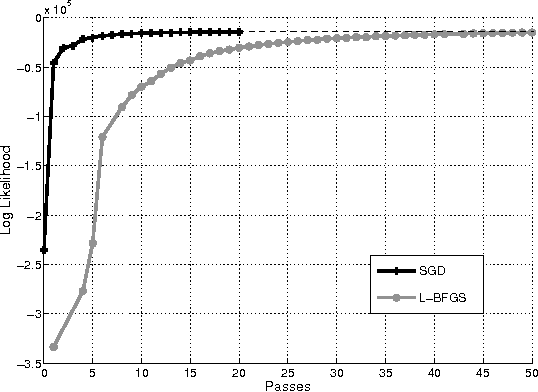
\includegraphics[height=2in]{stochastic.png}
    \begin{itemize}
      \item Use SGD for optimization
      \item compared SGD to L-BFGS
      \item \textbf{7x speedup} on WSJ15
    \end{itemize}
  \end{block}
\end{frame}

\begin{frame}
  \frametitle{Features}
  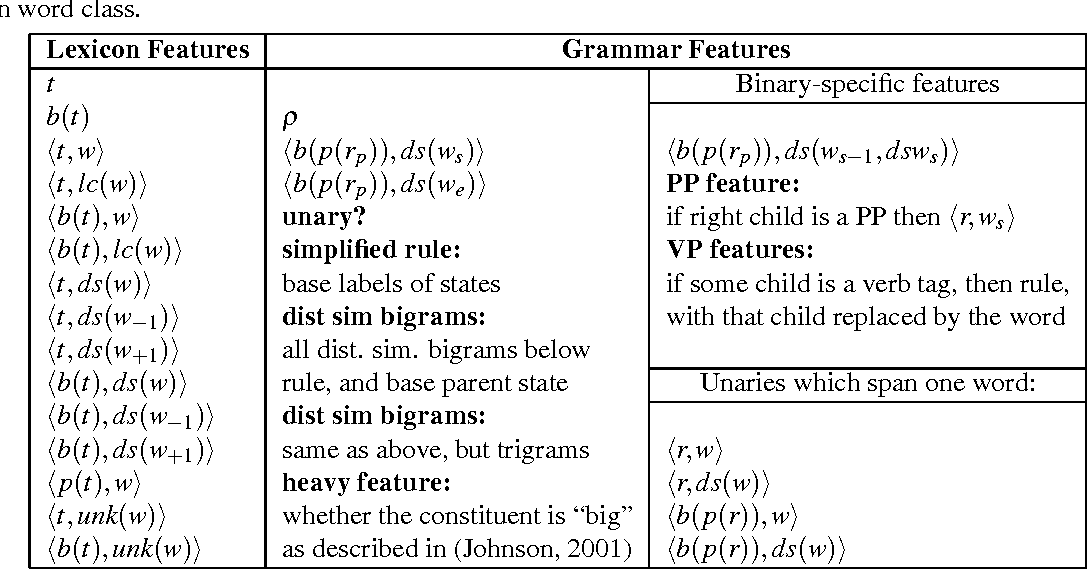
\includegraphics[height=2in]{features.png}
  \begin{itemize}
    \item Their model allowed them to incoperate "lexicon features" (words over tags) and
          "grammar features" (local subtrees and corresponding span/split)
    \item Features had to be tuned on sentences $\leq 15$ because $\leq 40$ was infesible
  \end{itemize}
\end{frame}
  
\begin{frame}
  \frametitle{Experiments}
  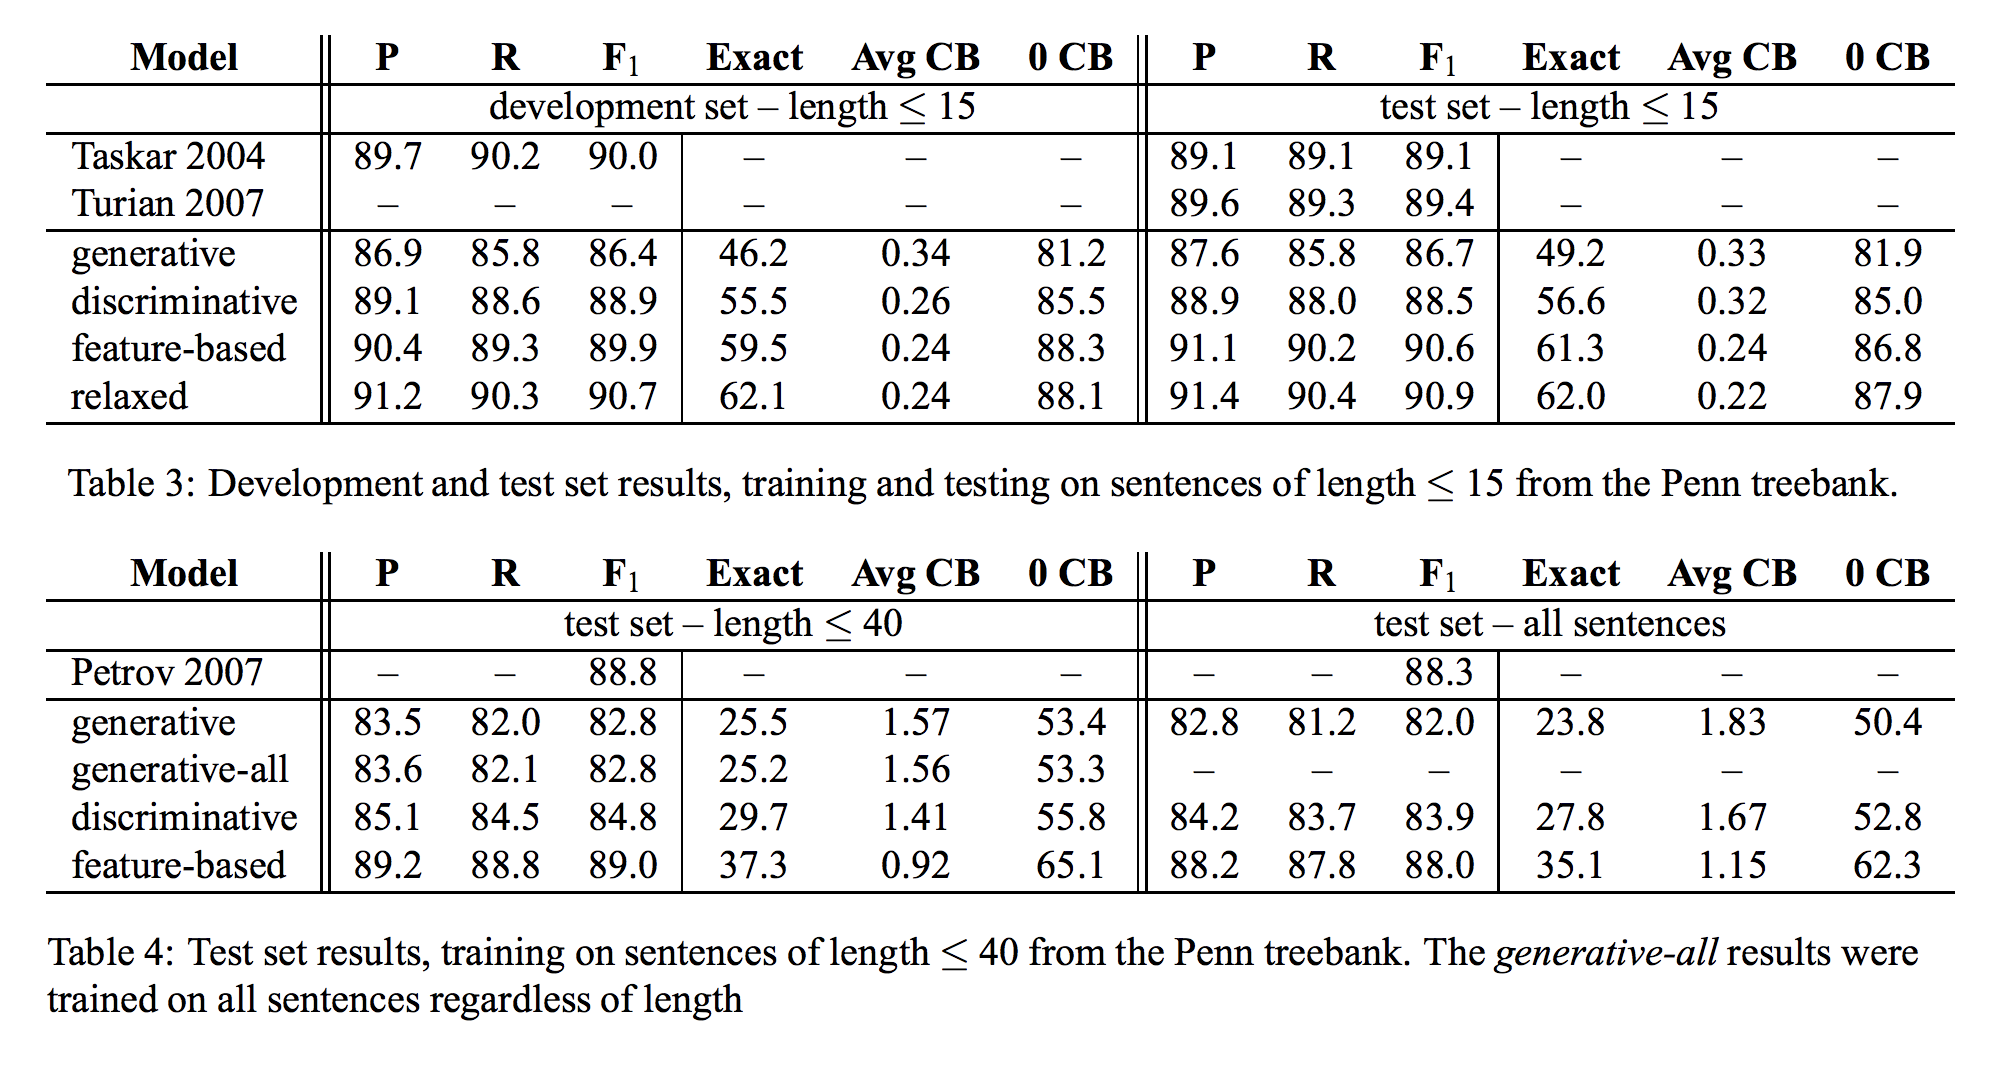
\includegraphics[height=2in]{results.png}

  \begin{itemize}
    \item Discriminatively trained model: Lexicon Featrues, no Grammer Features
    \item Feature-based model: Lexicon Featrues and Grammer Features
    \item Relaxed model: Feature model with rules not seen in training
  \end{itemize}
\end{frame}

\begin{frame}
  \frametitle{Experiments}
  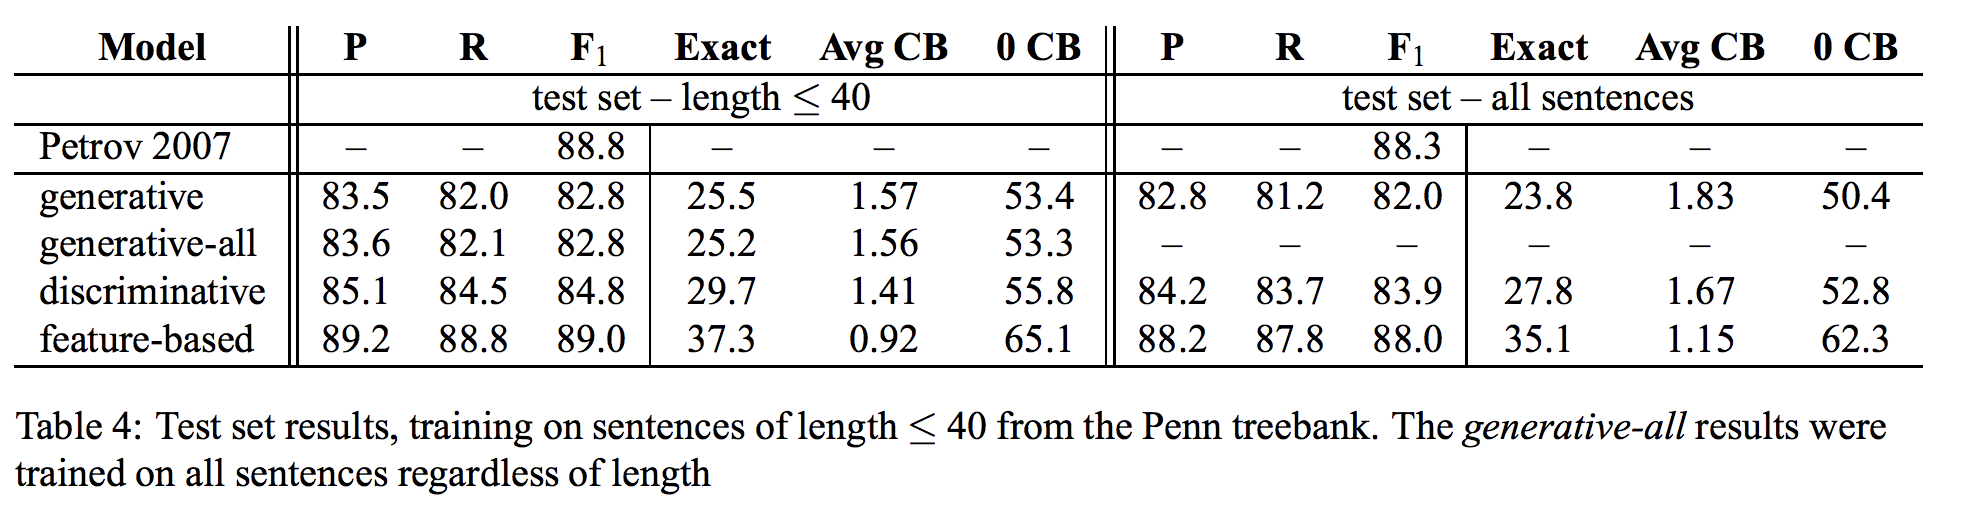
\includegraphics[height=1in]{resultsred.png}
  \begin{block}{Performance}
    \begin{itemize}
      \item On WSJ15: (20 passes)
        \begin{itemize}
          \item Discriminatively trained generative model (\textit{discriminative}):  \\
                1 machine; 3 gigabytes of RAM; 12 min/pass
          \item Feature-based model  (\textit{feature-based}):  \\
                1 machine; 3 gigabytes of RAM; 35 min/pass
        \end{itemize}
      \item On WSJ40: (10 passes)
        \begin{itemize}
          \item Discriminatively trained generative model (\textit{discriminative}): \\
                2 machines; 16 gigabytes of RAM each; 1 day/pass
          \item Feature-based model  (\textit{feature-based}):  \\
                4 machines; 16 gigabytes of RAM each; 3 day/pass
        \end{itemize}
    \end{itemize}
  \end{block}
\end{frame}


\begin{frame}
  \frametitle{Experiments}
  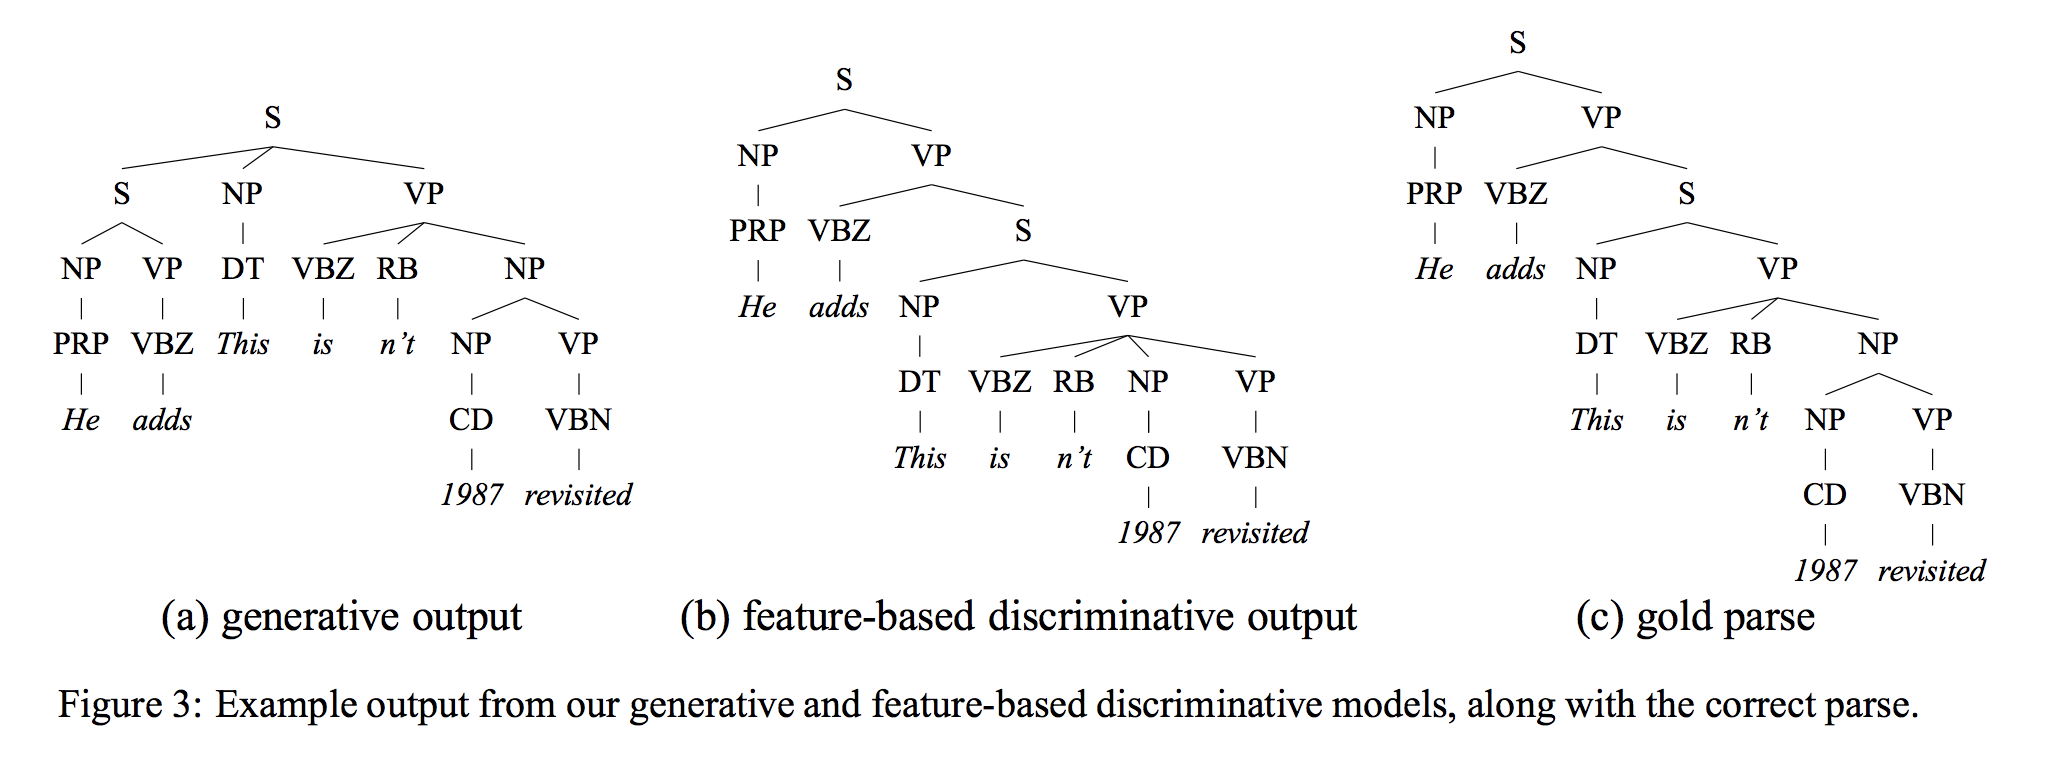
\includegraphics[height=1.5in]{trees.png}
  \begin{itemize}
    \item They highlight the models ability to capture the right-branching tendencies of English  \\
    \item Specifically the "heavy" feature encouraging long constituants at ends of sentences
  \end{itemize}
\end{frame}

\begin{frame}
  \frametitle{Impact}
  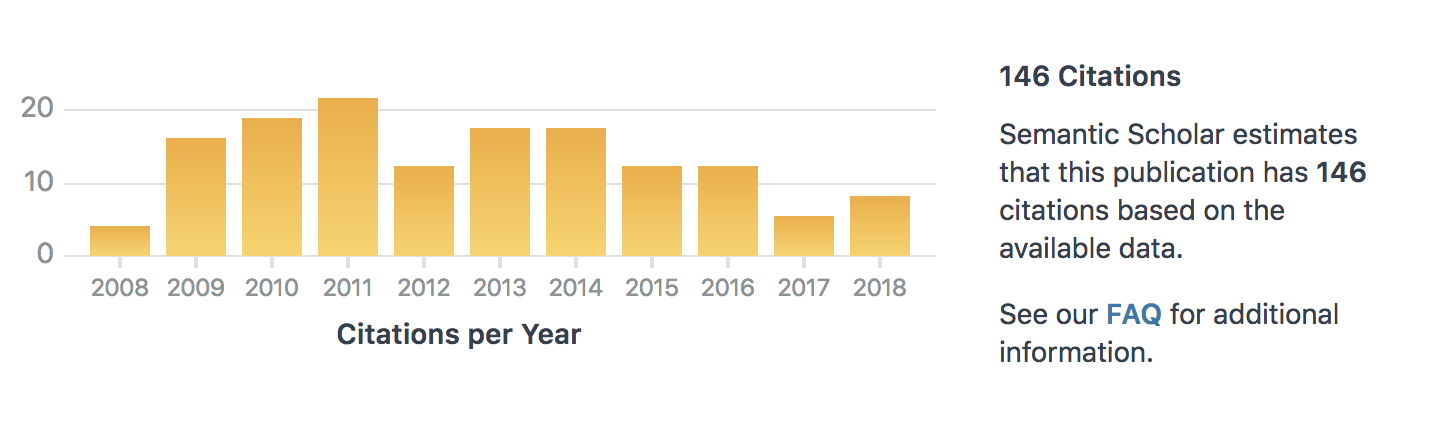
\includegraphics[height=1in]{citations.png}
  \begin{block}{Why was this work influential?}
    \begin{itemize}
      \item Defined a discriminative, feature based model that's simple, effective, and faster to
            train than previous methods.
      \item "Looking at how other tasks, such as named
            entity recognition and part-of-speech tagging, have
            evolved over time, it is clear that greater gains are to
            be gotten from developing better features than from
            better models."
            
    \end{itemize}
  \end{block}
\end{frame}

\begin{frame}
  \center{\huge Thanks! Question?}
\end{frame}

\end{document}
